\chapter{Altera Cyclone V VxWorks Boot} % Chapter title

\label{ch:materialandmethods} % For referencing the chapter elsewhere, use \autoref{ch:examples} 

%----------------------------------------------------------------------------------------

\section{Overview}
\label{overview}
The following figure depicts the typical boot flow: \\
\begin{figure}[h]
	\centering		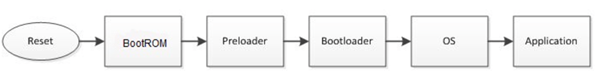
\includegraphics[width=0.8\textwidth]{img/bootschema1}
	\caption{Boot flow}
    	\label{fig:bootflow}
\end{figure}

Additional boot flows are possible, as shown in the following diagram:
\begin{figure}[h]
	\centering		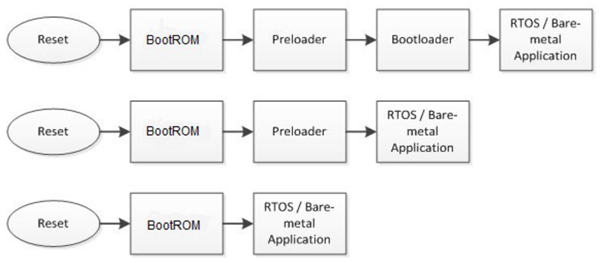
\includegraphics[width=0.8\textwidth]{img/bootschema2}
	\caption{Additional boot flow}
    	\label{fig:bootflow2}
\end{figure}

\textbf{The HPS boot} process starts when the processor is released from reset, and jumps to the reset vector address, located in the Boot ROM address space.\newline
Typically, the main responsibilities of the Boot ROM are: 
\begin{itemize}
\item Detect the selected boot source;
\item Perform minimal HPS initialization; 
\item Load the next boot stage (typically the Preloader) from Flash to OCRAM and jump to it.
\end{itemize}
The behavior of the Boot ROM is influenced by the BSEL and CSEL options (rev B, C).\\
Typical board switches layout found in the references.
\begin{figure}[h]
	\centering		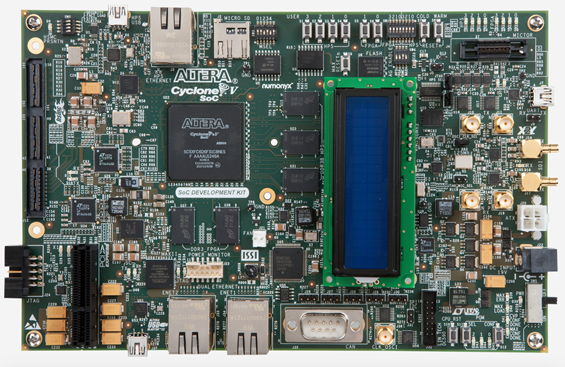
\includegraphics[width=0.8\textwidth]{img/ciclonv1}
	\caption{Altera Cyclon V}
    	\label{fig:ciclonv1}
\end{figure}
\begin{figure}[h]
	\centering		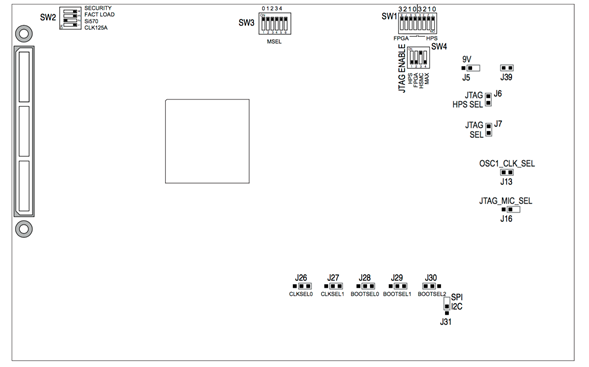
\includegraphics[width=0.8\textwidth]{img/ciclonv2}
	\caption{Altera Cyclon V switchs}
    	\label{fig:ciclonv2}
\end{figure}

\clearpage
\newpage

Our board. The switches are configured for FPGA Working Mode.
\begin{figure}[h]
	\centering		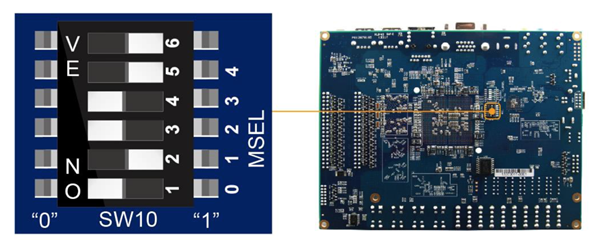
\includegraphics[width=0.8\textwidth]{img/ciclonv3}
	\caption{MSEL}
    	\label{fig:ciclonv3}
\end{figure}


Running Linux to check the correct configuration of the board switches.
\begin{itemize}
\item \textbf{What is necessary:}

\begin{enumerate}
\item SD card ( At least 4 gb);
\item Win32DiskImager.exe ( \url{http://sourceforge.net/projects/win32diskimager/} to flash the Linux Image on the SD; 
\item Pre-built SD Card Image ( \url{http://www.terasic.com/downloads/cd-rom/de1-soc/linux_BSP/DE1_SoC_SD.zip}.);
\item Putty.
\end{enumerate}

\item \textbf{What is inside the default image:}

\begin{enumerate}
\item SPL Pre-loader;
\item U-boot; 
\item Device Tree Blob;
\item Linux Kernel;
\item Linux Root File system.
\end{enumerate}

\item \textbf{MSEL CONFIGURATION}
\begin{figure}[h]
	\centering		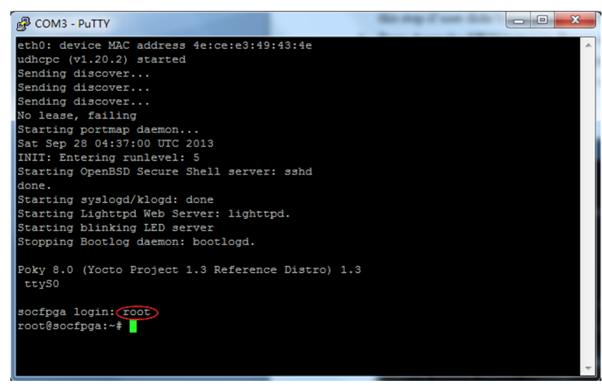
\includegraphics[width=0.8\textwidth]{img/putty1}
	\caption{Shown with Putty application}
    	\label{fig:putty}
\end{figure}
\begin{figure}[h]
	\centering		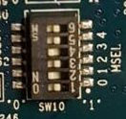
\includegraphics[width=0.3\textwidth]{img/msel}
	\caption{Msel switchs}
    	\label{fig:msel}
\end{figure}
\end{itemize}

\clearpage
\newpage
The preloader configures clocking, IOCSR, pinmuxing, DDRAM and loads the second-stage bootloader( like U-boot  or in our case the VxWorks bootloader ) into DDRAM.

\begin{figure}[h]
	\centering		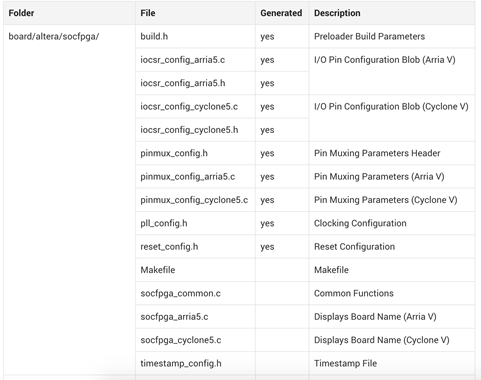
\includegraphics[width=0.8\textwidth]{img/folder}
	\caption{socfpga folder}
    	\label{fig:folder}
\end{figure}

\clearpage
\section{Preloader}
\label{preloader}

\begin{figure}[h]
	\centering		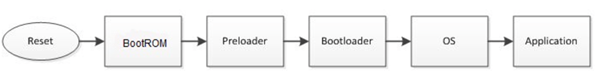
\includegraphics[width=0.8\textwidth]{img/bootschema1}
	\caption{Boot flow}
    	\label{fig:bootflow}
\end{figure}

The modifications made to the uboot-socfpga/board/altera/socfpga/build.h file are shown below in bolded text: 

\begin{lstlisting}[style=myCode]
/* Enable FAT partition support when booting from SDMMC. */ 
#define CONFIG_PRELOADER_FAT_SUPPORT (1)

/* When FAT partition support is enabled, this specifies the * FAT partition where the boot image is located. */
#define CONFIG_PRELOADER_FAT_BOOT_PARTITION (1)

/* When FAT partition supported is enabled, this specifies the * boot image filename within a FAT partition to be used as fatload payload.*/
#define CONFIG_PRELOADER_FAT_LOAD_PAYLOAD_NAME "bootloader.bin" 
\end{lstlisting}   

Another change where the preloader loads the FPGA file was made to the uboot-socfpga/include/configs/ socfpga\_common.h file:

\begin{lstlisting}[style=myCode]
/*  FPGA programming support with SPL FPGA RBF file source (with mkimage header) is located within the same  boot device which stored the subsequent boot image (U-Boot). */

/* enabled program the FPGA */
#define CONFIG_SPL_FPGA_LOAD 
\end{lstlisting} 

\clearpage
\section{Bootloader}
\label{bootloader}

\begin{figure}[h]
	\centering		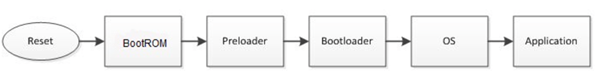
\includegraphics[width=0.8\textwidth]{img/bootschema1}
	\caption{Boot flow}
    	\label{fig:bootflow}
\end{figure}

We have built the  VxWorks bootrom file using Wind River tools and the alt\_soc\_gen5 BSP using the workbench of Wind River.
	
\begin{lstlisting}[style=myCode]
-A arm -T firmware -C none -O vxworks -a 0x08000040 -  e 0 -n "vxWorks bootloader for SoC FPGA" -d bootrom.bin  bootloader.bin 
\end{lstlisting} 

Finally we have put everything on the SD Card and we had tried to boot the system with no results.\\					
This method is described by the official documentation from the Intel/Altera site.  Also the software is provided.
\begin{figure}[h]
	\centering		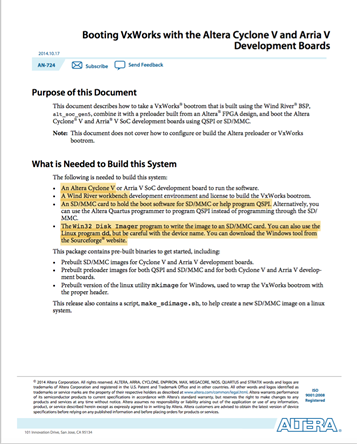
\includegraphics[width=0.6\textwidth]{img/bootguide}
	\caption{Boot cyclonV guide}
    	\label{fig:bootguide}
\end{figure}

\clearpage
\section{From scratch}
\label{Fromscratch}

\begin{figure}[h]
	\centering		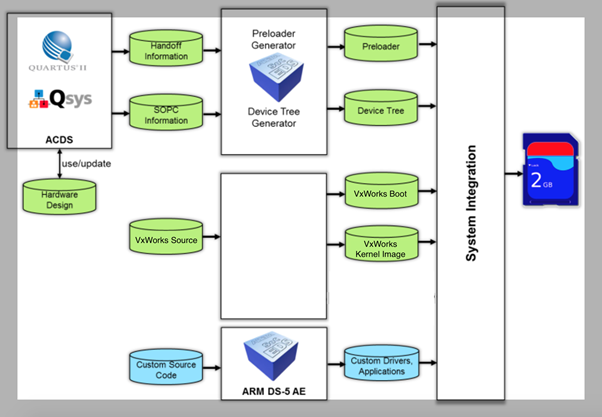
\includegraphics[width=0.6\textwidth]{img/fromscratch}
	\caption{From scratch}
    	\label{fig:fromscratch}
\end{figure}

\subsection{Compiling the Hardware Design}
\begin{figure}[h]
	\centering		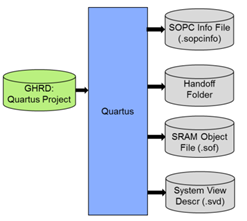
\includegraphics[width=0.4\textwidth]{img/ghrd}
	\caption{GHRD}
    	\label{fig:ghrd}
\end{figure}

\begin{figure}[h]
	\centering		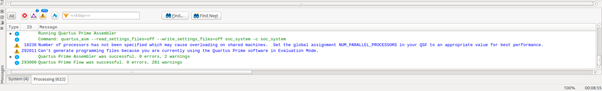
\includegraphics[width=0.8\textwidth]{img/quartuserror}
	\caption{Quartus Error}
    	\label{fig:quartuserror}
\end{figure}


\url{https://rocketboards.org/foswiki/view/Documentation/GSRDCompileHardwareDesign}.

\subsection{Compiling the Preloader}
\begin{figure}[h]
	\centering		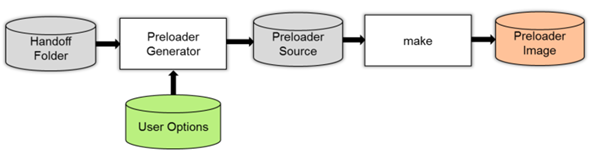
\includegraphics[width=0.8\textwidth]{img/schema}
	\caption{Compiling schema}
    	\label{fig:schema}
\end{figure}

\url{https://rocketboards.org/foswiki/view/Documentation/GSRDPreloader}.

\subsection{Device Tree}
The device tree is a data structure for describing hardware. 
Given the correct device tree, the same compiled kernel can support different hardware configurations within a wider architecture family.\\
For ARM, use of device trees has become mandatory for all new SoCs.\\
This can be seen as a remedy to the vast number of forks (of Linux and Das U-boot) that has historically been created to support (marginally) different ARM boards.\\

\begin{figure}[h]
	\centering		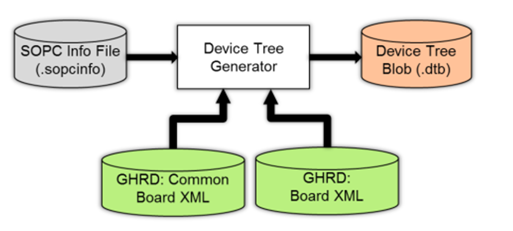
\includegraphics[width=0.6\textwidth]{img/devicetree}
	\caption{Device tree}
    	\label{fig:devicetree}
\end{figure}

\url{https://rocketboards.org/foswiki/view/Documentation/GSRDDeviceTreeGenerator}.

\subsection{Vivado}
We used Vivado on the workstation to build ….
We built the VxWorks image for the Cyclone V.
Building the device tree it gave an error, so we forced the output.\\ 
We put on the SD the image, the device tree and the bootloader.\\
We tried to boot but nothing showed up, neither with the forced device tree, nor with the .dts file already provided.\\

\begin{figure}[h]
	\centering		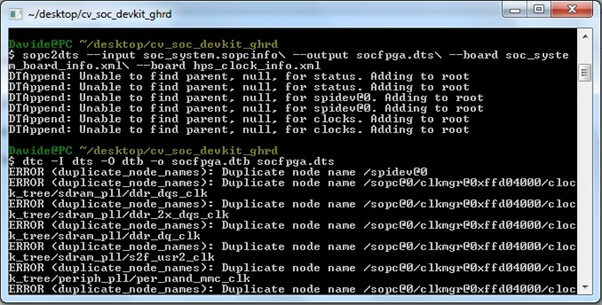
\includegraphics[width=0.6\textwidth]{img/devicetreeerror}
	\caption{Device tree error}
    	\label{fig:devicetreeerror}
\end{figure}





